% Copyright (c) 2026 CorrectBrain
% SPDX-License-Identifier: MIT

\PassOptionsToPackage{dvipsnames,svgnames,x11names}{xcolor}
\documentclass[tikz,border=8pt]{standalone}
\usetikzlibrary{arrows.meta,positioning,calc,shapes,shadows,decorations.pathmorphing,shapes.geometric,backgrounds,decorations.markings,decorations.pathreplacing,decorations.text,fit,shapes.misc,shapes.arrows,matrix,bending,3d,chains,intersections,shapes.symbols,svg.path,shapes.multipart,snakes,shapes.callouts,angles,quotes}
\providecolor{gold}{RGB}{212,175,55}
\providecolor{silver}{RGB}{192,192,192}
\providecolor{bronze}{RGB}{205,127,50}
\providecolor{darkblue}{RGB}{0,0,139}
\providecolor{lightblue}{RGB}{173,216,230}
\providecolor{darkgreen}{RGB}{0,100,0}
\providecolor{lightgreen}{RGB}{144,238,144}
\providecolor{darkred}{RGB}{139,0,0}
\providecolor{navy}{RGB}{0,0,128}
\providecolor{skyblue}{RGB}{135,206,235}
\providecolor{beige}{RGB}{245,245,220}
\providecolor{cream}{RGB}{255,253,208}
\usepackage{amsmath}
\usepackage{amssymb}
\usepackage{fontawesome5}
\usetikzlibrary{fadings,shadows.blur,patterns,patterns.meta}

\providecolor{gold}{RGB}{212,175,55}
\providecolor{silver}{RGB}{192,192,192}
\providecolor{bronze}{RGB}{205,127,50}
\providecolor{darkblue}{RGB}{0,0,139}
\providecolor{lightblue}{RGB}{173,216,230}
\providecolor{darkgreen}{RGB}{0,100,0}
\providecolor{lightgreen}{RGB}{144,238,144}
\providecolor{darkred}{RGB}{139,0,0}
\providecolor{navy}{RGB}{0,0,128}
\providecolor{skyblue}{RGB}{135,206,235}
\providecolor{beige}{RGB}{245,245,220}
\providecolor{cream}{RGB}{255,253,208}
\usepackage{amsmath}
\usepackage{amssymb}
\usepackage{fontawesome5}


\providecolor{gold}{RGB}{212,175,55}
\providecolor{silver}{RGB}{192,192,192}
\providecolor{bronze}{RGB}{205,127,50}
\providecolor{darkblue}{RGB}{0,0,139}
\providecolor{lightblue}{RGB}{173,216,230}
\providecolor{darkgreen}{RGB}{0,100,0}
\providecolor{lightgreen}{RGB}{144,238,144}
\providecolor{darkred}{RGB}{139,0,0}
\providecolor{navy}{RGB}{0,0,128}
\providecolor{skyblue}{RGB}{135,206,235}
\providecolor{beige}{RGB}{245,245,220}
\providecolor{cream}{RGB}{255,253,208}
\usepackage{amsmath}
\usepackage{amssymb}
\usepackage{fontawesome5}

\providecolor{gold}{RGB}{212,175,55}
\providecolor{silver}{RGB}{192,192,192}
\providecolor{bronze}{RGB}{205,127,50}
\providecolor{darkblue}{RGB}{0,0,139}
\providecolor{lightblue}{RGB}{173,216,230}
\providecolor{darkgreen}{RGB}{0,100,0}
\providecolor{lightgreen}{RGB}{144,238,144}
\providecolor{darkred}{RGB}{139,0,0}
\providecolor{navy}{RGB}{0,0,128}
\providecolor{skyblue}{RGB}{135,206,235}
\providecolor{beige}{RGB}{245,245,220}
\providecolor{cream}{RGB}{255,253,208}
\providecolor{NavyBlue}{RGB}{0,0,128}
\providecolor{MidnightBlue}{RGB}{25,25,112}
\providecolor{SkyBlue}{RGB}{135,206,235}
\providecolor{DarkSlateGray}{RGB}{47,79,79}
\usepackage{amsmath}
\usepackage{amssymb}
\usepackage{fontawesome5}

\usepackage{tikz}
\usepackage{xcolor}

\definecolor{accentR}{RGB}{220, 53, 69}
\definecolor{accentP}{RGB}{111, 66, 193}

% -------------------------------------------------------------
% REUSABLE HYPER-REALISTIC VECTOR LANDSCAPE ARTWORK
% Native Coordinate Space: [0, 8] in X, [0, 3] in Y
% Focal Subject Anchor: (4.0, 0.7)
% -------------------------------------------------------------
\newcommand{\drawLandscapeArtwork}{%
  % Sky Gradient: Deep dusk navy to atmospheric soft cyan
  \shade[top color=MidnightBlue!90!NavyBlue, bottom color=SkyBlue!35!white] (0,0) rectangle (8,3);

  % Subtle Vector Cloud Layers
  \path[fill=white, opacity=0.15] (0, 2.5) .. controls (2, 2.7) and (3, 2.3) .. (5, 2.6) .. controls (6.5, 2.8) and (7.5, 2.4) .. (8, 2.5) -- (8, 3) -- (0, 3) -- cycle;
  \path[fill=white, opacity=0.08] (0, 2.1) .. controls (1.5, 2.3) and (3.5, 1.9) .. (6, 2.2) .. controls (7, 2.4) .. (8, 2.1) -- (8, 2.4) -- (0, 2.4) -- cycle;

  % Realistic Radiant Celestial Body with Atmospheric Glow
  \fill[orange!30!yellow, opacity=0.25] (6.6, 2.2) circle (0.7);
  \fill[orange!50!yellow, opacity=0.45] (6.6, 2.2) circle (0.42);
  \fill[yellow!80!white, opacity=0.85] (6.6, 2.2) circle (0.22);
  \fill[white] (6.6, 2.2) circle (0.12);

  % Distant Mountain Range (Layer 1 - Atmospheric Blue Haze)
  \fill[top color=MidnightBlue!65!DarkSlateGray, bottom color=MidnightBlue!90!black]
    (0,0) -- (0, 1.2)
    .. controls (1.0, 1.8) and (1.8, 1.3) .. (2.8, 2.3)
    .. controls (3.5, 1.7) and (4.2, 2.1) .. (5.2, 1.5)
    .. controls (6.0, 2.4) and (6.8, 1.8) .. (7.6, 2.2)
    -- (8, 1.8) -- (8, 0) -- cycle;

  % Snow Caps on Distant Peaks
  \path[fill=white!85!SkyBlue, opacity=0.75]
    (2.8, 2.3) -- (2.5, 1.9) .. controls (2.7, 1.85) .. (2.9, 1.95) -- (3.1, 1.8) -- cycle;
  \path[fill=white!85!SkyBlue, opacity=0.75]
    (7.6, 2.2) -- (7.3, 1.85) .. controls (7.5, 1.8) .. (7.7, 1.9) -- (7.85, 1.85) -- cycle;

  % Mid-Distance Mountain Ridge (Layer 2 - Detailed Vector Facets)
  \fill[top color=NavyBlue!80!black, bottom color=MidnightBlue!95!black]
    (0,0) -- (0, 0.9)
    -- (1.2, 1.7) -- (2.2, 0.9)
    -- (3.8, 2.2) -- (4.8, 1.2)
    -- (6.2, 2.0) -- (7.2, 1.1) -- (8, 1.5) -- (8, 0) -- cycle;

  % Ridge Shading & Depth Shadows
  \fill[black!40, opacity=0.55]
    (1.2, 1.7) -- (2.2, 0.9) -- (1.5, 0.7) -- cycle;
  \fill[black!40, opacity=0.55]
    (3.8, 2.2) -- (4.8, 1.2) -- (4.1, 0.9) -- cycle;
  \fill[black!40, opacity=0.55]
    (6.2, 2.0) -- (7.2, 1.1) -- (6.6, 0.8) -- cycle;

  % Snow Caps on Mid-Range Peaks
  \path[fill=white!95!cyan]
    (3.8, 2.2) -- (3.4, 1.8) -- (3.7, 1.85) -- (3.9, 1.75) -- (4.2, 1.8) -- cycle;
  \path[fill=white!95!cyan]
    (6.2, 2.0) -- (5.9, 1.7) -- (6.1, 1.75) -- (6.3, 1.68) -- (6.5, 1.72) -- cycle;

  % Foreground Mountain Peaks & Sharp Slate Ridges (Layer 3)
  \fill[top color=DarkSlateGray!90!black, bottom color=black!95!MidnightBlue]
    (0,0) -- (0, 0.6)
    -- (0.8, 1.3) -- (1.8, 0.5)
    -- (2.6, 1.1) -- (3.5, 0.4)
    -- (4.0, 1.0) -- (4.8, 0.35)
    -- (5.8, 1.2) -- (6.8, 0.4)
    -- (7.5, 0.9) -- (8, 0.5) -- (8, 0) -- cycle;

  % Sharp Vector Foreground Snowcaps
  \path[fill=white]
    (0.8, 1.3) -- (0.6, 1.0) -- (0.9, 1.05) -- (1.0, 0.95) -- cycle;
  \path[fill=white]
    (5.8, 1.2) -- (5.5, 0.95) -- (5.8, 1.0) -- (6.1, 0.9) -- cycle;

  % Alpine Pine Forest Silhouettes on Valley Floor
  \foreach \tx/\ty in {0.2/0.2, 0.5/0.25, 0.9/0.18, 1.4/0.15, 2.0/0.22, 2.5/0.18, 3.2/0.12, 4.6/0.15, 5.2/0.18, 5.5/0.22, 6.4/0.15, 7.0/0.2, 7.6/0.18} {
    \fill[black!95!MidnightBlue] (\tx, \ty) -- (\tx-0.08, \ty-0.18) -- (\tx+0.08, \ty-0.18) -- cycle;
    \fill[black!95!MidnightBlue] (\tx, \ty+0.08) -- (\tx-0.06, \ty-0.06) -- (\tx+0.06, \ty-0.06) -- cycle;
  }

  % Valley Terrain Floor Base
  \fill[black!95!MidnightBlue] (0,0) rectangle (8, 0.08);

  % High-Contrast Tech Beacon / Alpine Cabin at Focal Point (4.0, 0.7)
  \fill[accentR, opacity=0.25] (4.0, 0.7) circle (0.45);
  \fill[accentR, opacity=0.45] (4.0, 0.7) circle (0.28);
  \fill[black!95] (3.88, 0.55) rectangle (4.12, 0.75);
  \fill[accentR!80!black] (3.84, 0.75) -- (4.0, 0.88) -- (4.16, 0.75) -- cycle;
  \fill[yellow!90!white] (3.95, 0.62) rectangle (4.05, 0.72);
  \fill[accentR] (4.0, 0.7) circle (0.16);
  \fill[white] (4.0, 0.7) circle (0.05);
}

\begin{document}
\begin{tikzpicture}[x=1cm, y=1cm]

% ---------------- GLOBAL CANVAS & STRICT WHITE BACKGROUND ----------------
\path[fill=white] (-1, -7) rectangle (23, 26);

% ---------------- TITLE AND HEADER LAYOUT ----------------
\node[font=\Huge\bfseries\sffamily, color=black!90, align=center, text width=21cm] at (11, 24.5) {Art Direction: Mathematical Framing Boundaries};
\node[font=\Large\ttfamily, color=black!75, align=center, text width=21cm] at (11,22.1838) {How \texttt{<picture>} dynamically remaps image intrinsic dimensions to mobile endpoint constraints.};
\node[font=\Large\bfseries, color=black!85, align=center, text width=21cm] at (11,20.6838) {Server-Side Intrinsic Image Assets};


% ---------------- TOP SECTION: SERVER-SIDE ASSETS ----------------

% --- Asset 1: wide.jpg (8:3 Ratio) ---
% Dimension Indicators
\draw[thick, black!60] (2, 18.7) -- (2, 18.9) -- (10, 18.9) -- (10, 18.7);
\node[font=\small\ttfamily\bfseries, color=black!85] at (6, 19.2) {Intrinsic: 2400px (W) x 900px (H) [8:3]};
\draw[thick, black!60] (1.8, 15.5) -- (1.6, 15.5) -- (1.6, 18.5) -- (1.8, 18.5);
\node[font=\small\ttfamily\bfseries, color=black!85, rotate=90] at (1.3, 17.0) {900px};

% Asset 1 Vector Rendering (Bounds: 2 to 10 wide, 15.5 to 18.5 high)
\begin{scope}
  \clip (2, 15.5) rectangle (10, 18.5);
  \begin{scope}[shift={(2, 15.5)}]
    \drawLandscapeArtwork
  \end{scope}
\end{scope}
\draw[line width=1.2pt, black!75, rounded corners=1pt] (2, 15.5) rectangle (10, 18.5);

% Focal Subject Reticle & Mapping (Absolute Center: 6.0, 16.2)
\draw[line width=1.5pt, accentR, dashed] (5.6, 15.8) rectangle (6.4, 16.6);
\draw[line width=1.2pt, accentR] (5.5, 16.2) -- (5.6, 16.2) (6.4, 16.2) -- (6.5, 16.2) (6.0, 15.7) -- (6.0, 15.8) (6.0, 16.6) -- (6.0, 16.7);
\node[font=\footnotesize\bfseries, color=accentR, inner sep=2pt] (focal1) at (6, 15.1) {Focal Subject};
\draw[line width=1.2pt, accentR] (6.0, 15.7) -- (focal1.north);


% --- Asset 2: tight-crop.jpg (1:1 Ratio) ---
% Dimension Indicators
\draw[thick, black!60] (15, 18.7) -- (15, 18.9) -- (18, 18.9) -- (18, 18.7);
\node[font=\small\ttfamily\bfseries, color=black!85] at (16.5, 19.2) {Intrinsic: 900px (W) x 900px (H) [1:1]};
\draw[thick, black!60] (14.8, 15.5) -- (14.6, 15.5) -- (14.6, 18.5) -- (14.8, 18.5);
\node[font=\small\ttfamily\bfseries, color=black!85, rotate=90] at (14.3, 17.0) {900px};

% Asset 2 Vector Rendering (Mathematically exact 1:1 clone of Asset 1 from X=4.5 to X=7.5)
\begin{scope}
  \clip (15, 15.5) rectangle (18, 18.5);
  \begin{scope}[shift={(12.5, 15.5)}]
    \drawLandscapeArtwork
  \end{scope}
\end{scope}
\draw[line width=1.2pt, black!75, rounded corners=1pt] (15, 15.5) rectangle (18, 18.5);

% Focal Subject Reticle (Absolute Center: 16.5, 16.2)
\draw[line width=1.5pt, accentP, dashed] (16.1, 15.8) rectangle (16.9, 16.6);
\draw[line width=1.2pt, accentP] (16.0, 16.2) -- (16.1, 16.2) (16.9, 16.2) -- (17.0, 16.2) (16.5, 15.7) -- (16.5, 15.8) (16.5, 16.6) -- (16.5, 16.7);
\node[font=\footnotesize\bfseries, color=accentP, inner sep=2pt] (focal2) at (16.5, 15.1) {Focal Subject};
\draw[line width=1.2pt, accentP] (16.5, 15.7) -- (focal2.north);


% ---------------- BROWSER PRE-PARSER & MECHANICAL FLOW LAYER ----------------
\draw[draw=MidnightBlue!40, fill=MidnightBlue!2, drop shadow={opacity=0.03}, dashed, line width=1pt, rounded corners=8pt] (0.8, 11.6) rectangle (21.2, 14.6);
\node[font=\scriptsize\sffamily\bfseries, color=black!60, fill=white, inner sep=6pt, anchor=center] at (11, 14.6) {\faCogs\quad BROWSER RENDERING ENGINE / PRE-PARSER LAYER};

% White Masking Nodes to Prevent Dashed Border Crossings Collisions
\node[fill=white, minimum width=8mm, minimum height=4mm, inner sep=0pt] at (6, 14.6) {};
\node[fill=white, minimum width=8mm, minimum height=4mm, inner sep=0pt] at (16.5, 14.6) {};
\node[fill=white, minimum width=8mm, minimum height=4mm, inner sep=0pt] at (6, 11.6) {};
\node[fill=white, minimum width=8mm, minimum height=4mm, inner sep=0pt] at (16.5, 11.6) {};

% Left Flow Nodes (Standard Pipeline)
\node[fill=white, draw=black!25, line width=0.8pt, rounded corners=3pt, font=\scriptsize\sffamily, align=center, inner sep=4pt, text width=5cm] (L1) at (6, 13.8) {HTML Preload Scanner\\[2pt] \texttt{<img>} src identified};
\node[fill=white, draw=black!25, line width=0.8pt, rounded corners=3pt, font=\scriptsize\sffamily, align=center, inner sep=4pt, text width=5cm] (L2) at (6, 12.4) {Default CSS Flow\\[2pt] (\texttt{max-width: 100\%})};

% Right Flow Nodes (Art Direction Override Pipeline)
\node[fill=white, draw=accentP!50, line width=0.8pt, rounded corners=3pt, font=\scriptsize\sffamily, text=accentP, align=center, inner sep=4pt, text width=6.5cm] (R1) at (16.5, 13.8) {Pre-parser Evaluator\\[2pt] \texttt{<source media="(max-width: 600px)">}};
\node[fill=white, draw=accentP, line width=1.2pt, rounded corners=3pt, font=\scriptsize\sffamily\bfseries, text=accentP, align=center, inner sep=4pt, text width=6.5cm] (R2) at (16.5, 12.4) {Media Match: \texttt{(max-width: 600px)}\\[2pt] Fetch \texttt{tight-crop.jpg}};

% Left Flow Arrows
\draw[-Stealth=3mm, line width=1.8pt, dashed, gray!60] (focal1.south) -- (L1.north);
\draw[-Stealth=3mm, line width=1.8pt, dashed, gray!60] (L1.south) -- (L2.north);
\draw[-Stealth=3mm, line width=1.8pt, dashed, gray!60] (L2.south) -- (6, 8.0);

% Right Flow Arrows
\draw[-Stealth=3mm, line width=1.8pt, dashed, accentP] (focal2.south) -- (R1.north);
\draw[-Stealth=3mm, line width=1.8pt, dashed, accentP] (R1.south) -- (R2.north);
\draw[-Stealth=3mm, line width=1.8pt, dashed, accentP] (R2.south) -- (16.5, 8.0);


% ---------------- BOTTOM SECTION: MOBILE ENDPOINTS ----------------
\node[font=\Large\bfseries, color=black!85, align=center] at (11, 10.0) {Mobile Endpoint Rendering\\[2pt] (Viewport Width = 400px)};

% ==================== PHONE 1: STANDARD max-width: 100% ====================
% Modern Smartphone Chassis (Center X = 6.0)
\fill[black!85, rounded corners=14pt] (3.8, -1.0) rectangle (8.2, 8.0);
\draw[black!60, line width=0.8pt, rounded corners=14pt] (3.8, -1.0) rectangle (8.2, 8.0);
\fill[white, rounded corners=6pt] (4.0, -0.7) rectangle (8.0, 7.7);

% Browser Top Bar Simulator
\fill[black!6] (4.0, 7.2) rectangle (8.0, 7.7);

% Phone 1 Rendered Image (Math: 4.0 Width x 1.5 Height -> 8:3 Exact Ratio)
\begin{scope}
  \clip (4.0, 6.2) rectangle (8.0, 7.7);
  \begin{scope}[shift={(4.0, 6.2)}, scale=0.5]
    \drawLandscapeArtwork
  \end{scope}
\end{scope}
\draw[line width=0.8pt, black!50] (4.0, 6.2) rectangle (8.0, 7.7);

% Dynamically Overlapping Camera Island / Notch
\fill[black!95, rounded corners=4pt] (5.3, 7.35) rectangle (6.7, 7.65);
\fill[black!70] (5.5, 7.5) circle (0.05);

% Squashed Subject Reticle on Phone 1 (Scaled to 0.5x intrinsic)
\draw[line width=1pt, accentR, dashed] (5.8, 6.35) rectangle (6.2, 6.75);

% Dimension Bracket
\draw[thick, accentR!60] (4.1, 6.0) -- (4.1, 5.85) -- (7.9, 5.85) -- (7.9, 6.0);

% Zero-Overlap Dimension & Scale Label (Strict anchor=north)
\node[font=\small\bfseries, color=accentR, align=center, text width=3.6cm, anchor=north] at (6.0, 5.75) {Rendered W: 400px\\(Scale 0.16x)};

% Mobile Browser Content Wireframe (Strict Screen Area Clip)
\begin{scope}
  \clip (4.0, -0.7) rectangle (8.0, 7.2);
  \fill[black!20, rounded corners=1.5pt] (4.3, 4.0) rectangle (7.7, 4.2);
  \fill[black!10, rounded corners=1pt] (4.3, 3.65) rectangle (7.5, 3.8);
  \fill[black!10, rounded corners=1pt] (4.3, 3.3) rectangle (7.7, 3.45);
  \fill[black!10, rounded corners=1pt] (4.3, 2.95) rectangle (6.8, 3.1);
  \fill[black!10, rounded corners=1pt] (4.3, 2.6) rectangle (7.6, 2.75);
  \fill[black!10, rounded corners=1pt] (4.3, 2.25) rectangle (6.0, 2.4);
\end{scope}

% Home Indicator Bar
\fill[black!30, rounded corners=1.5pt] (5.4, -0.55) rectangle (6.6, -0.45);

% Phone 1 Mathematical Annotation Box
\node[draw=accentR, line width=1.5pt, fill=white, rounded corners=6pt, drop shadow={opacity=0.1, shadow xshift=2pt, shadow yshift=-2pt}, text width=6.5cm, inner sep=10pt, align=center] at (6, -4.0) {
    \textbf{\color{accentR}\large Failure of \texttt{max-width: 100\%}}\\[6pt]
    $\text{Scale} = \frac{\text{Viewport W (400px)}}{\text{Intrinsic W (2400px)}} = 0.166$\\[6pt]
    The focal subject is mechanically reduced to 16\% of its intrinsic width. The framing boundary is broken and legibility is completely lost.
};


% ==================== PHONE 2: PICTURE/SOURCE ART DIRECTION ====================
% Modern Smartphone Chassis (Center X = 16.5)
\fill[black!85, rounded corners=14pt] (14.3, -1.0) rectangle (18.7, 8.0);
\draw[black!60, line width=0.8pt, rounded corners=14pt] (14.3, -1.0) rectangle (18.7, 8.0);
\fill[white, rounded corners=6pt] (14.5, -0.7) rectangle (18.5, 7.7);

% Browser Top Bar Simulator
\fill[black!6] (14.5, 7.2) rectangle (18.5, 7.7);

% Phone 2 Rendered Image (Math: 4.0 Width x 4.0 Height -> 1:1 Exact Ratio)
\begin{scope}
  \clip (14.5, 3.7) rectangle (18.5, 7.7);
  \begin{scope}[shift={(11.166667, 3.7)}, scale=1.3333333]
    \drawLandscapeArtwork
  \end{scope}
\end{scope}
\draw[line width=0.8pt, black!50] (14.5, 3.7) rectangle (18.5, 7.7);

% Dynamically Overlapping Camera Island / Notch
\fill[black!95, rounded corners=4pt] (15.8, 7.35) rectangle (17.2, 7.65);
\fill[black!70] (16.0, 7.5) circle (0.05);

% Preserved & Scaled Focal Subject Reticle on Phone 2 (Center: 16.5, 4.63)
\draw[line width=1.5pt, accentP, dashed] (15.967, 4.1) rectangle (17.033, 5.167);

% Dimension Bracket
\draw[thick, accentP!60] (14.6, 3.5) -- (14.6, 3.35) -- (18.4, 3.35) -- (18.4, 3.5);

% Zero-Overlap Dimension & Scale Label (Strict anchor=north)
\node[font=\small\bfseries, color=accentP, align=center, text width=3.6cm, anchor=north] at (16.5, 3.25) {Rendered W: 400px\\(Scale 0.44x)};

% Mobile Browser Content Wireframe (Strict Screen Area Clip)
\begin{scope}
  \clip (14.5, -0.7) rectangle (18.5, 7.2);
  \fill[black!20, rounded corners=1.5pt] (14.8, 1.5) rectangle (18.2, 1.7);
  \fill[black!10, rounded corners=1pt] (14.8, 1.15) rectangle (18.0, 1.3);
  \fill[black!10, rounded corners=1pt] (14.8, 0.8) rectangle (18.2, 0.95);
  \fill[black!10, rounded corners=1pt] (14.8, 0.45) rectangle (17.3, 0.6);
  \fill[black!10, rounded corners=1pt] (14.8, 0.1) rectangle (18.1, 0.25);
  \fill[black!10, rounded corners=1pt] (14.8, -0.25) rectangle (16.5, -0.1);
\end{scope}

% Home Indicator Bar
\fill[black!30, rounded corners=1.5pt] (15.9, -0.55) rectangle (17.1, -0.45);

% Phone 2 Mathematical Annotation Box
\node[draw=accentP, line width=1.5pt, fill=white, rounded corners=6pt, drop shadow={opacity=0.1, shadow xshift=2pt, shadow yshift=-2pt}, text width=6.5cm, inner sep=10pt, align=center] at (16.5, -4.0) {
    \textbf{\color{accentP}\large Success of Art Direction}\\[6pt]
    $\text{Scale} = \frac{\text{Viewport W (400px)}}{\text{Crop W (900px)}} = 0.444$\\[6pt]
    The \texttt{<source>} overrides standard flow and enforces a new intrinsic boundary box. The subject is mathematically preserved, rendering $\approx 7\times$ larger in area.
};

\end{tikzpicture}
\end{document}
